%% -*- coding: utf-8 -*-
\documentclass[14pt,a4paper]{scrartcl} 
\usepackage[utf8]{inputenc}
\usepackage[english,russian]{babel}
\usepackage{indentfirst}
\usepackage{misccorr}
\usepackage{graphicx}
\usepackage{amsmath}
\begin{document}
\tableofcontents
\newpage
\section{Введение}
Для разработки алгоритма использовалась среда разработки Visual Studio (в дальнейшем VS) на языке прогроммирования С++. При открытии VS запускается следующее окно (рисунок 1):
\begin{figure}[h!]
    \centering
    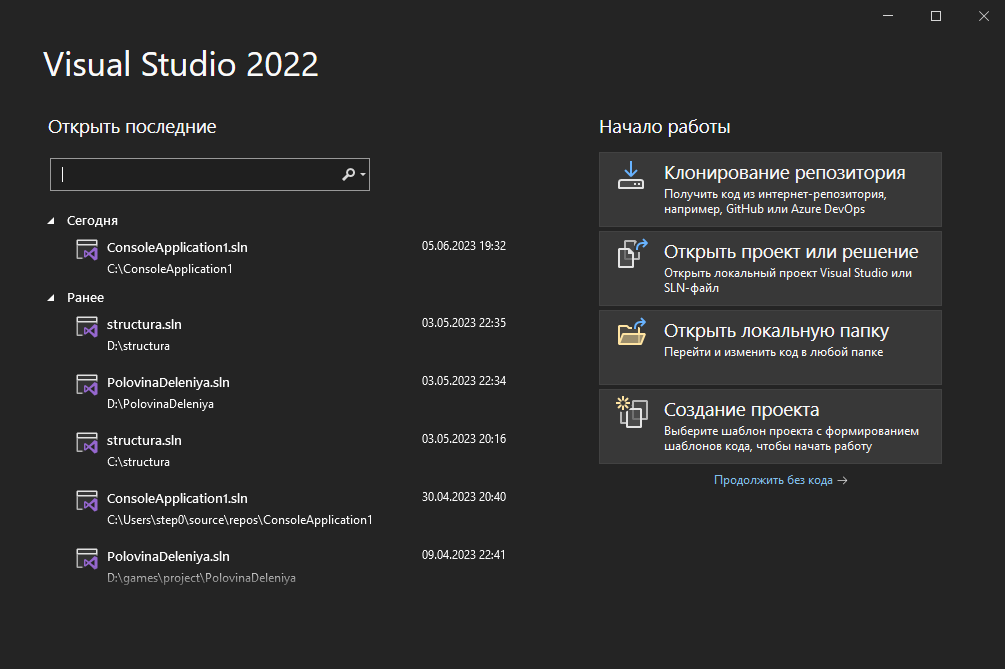
\includegraphics [width=0.9\textwidth]{pic1}\\
    \caption{Окно запуска проектов Visual Studio}
    \label{fig:pic1}
\end{figure}

\newpage

Для отрытия проекта необходимо кликнуть на нужное наименование после чего проект благополучно запуститься и можно начинать редактирование и компиляцию кода (рисунок 2): 

\begin{figure}[h!]
    \centering
    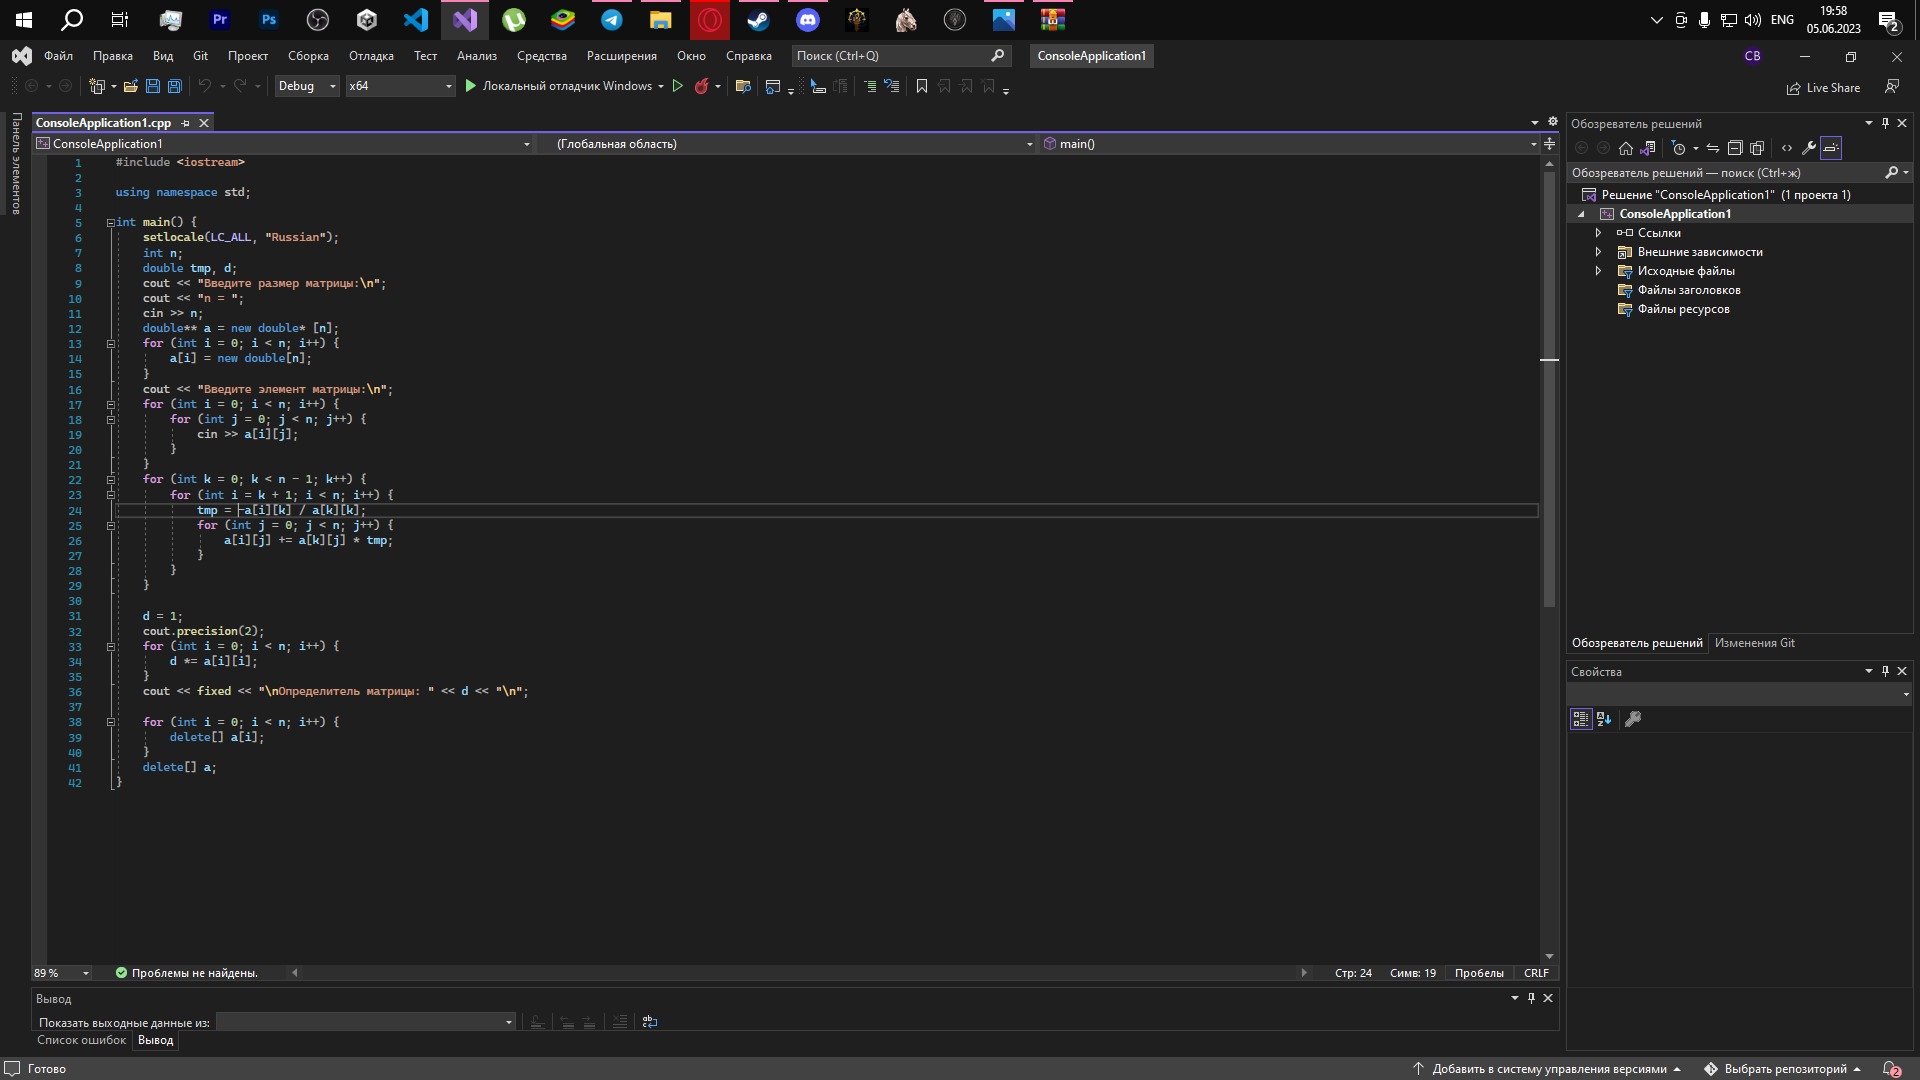
\includegraphics [width=0.9\textwidth]{pic2}\\
    \caption{Окно проекта Visual Studio}
    \label{fig:pic2}
\end{figure}

\newpage
\section{Работа программы}
На рисунке 2 можно увидеть алгоритм решения задачи на нахождение определителя матрицы методом Гаусса. Результат его работы отображён на рисунке 3:

\begin{figure}[h!]
    \centering
    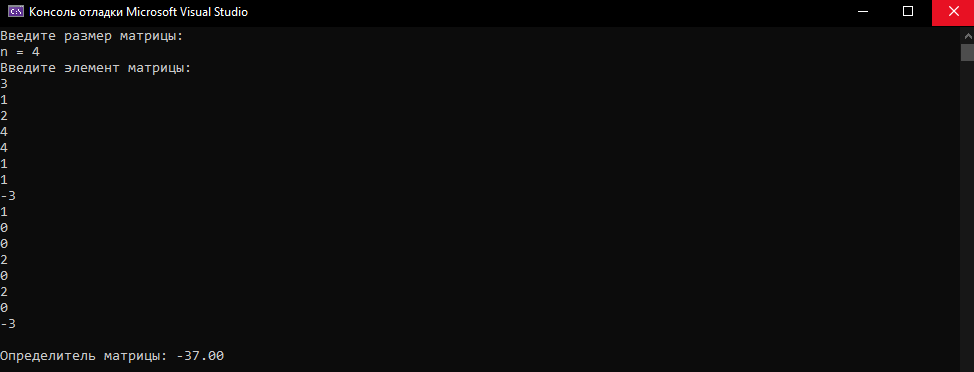
\includegraphics [width=0.9\textwidth]{pic3}\\
    \caption{Окно проекта Visual Studio}
    \label{fig:pic3}
\end{figure}

\newpage
\section{Список используемой литературы}

\begin{enumerate}

    \item Оосновы алгоритмизации и программирования, Т.А. Жданова, Ю.С. Бузыкова, 2011. - 59 с.
\end{enumerate}

\end{document}
